%% LyX 1.6.4 created this file.  For more info, see http://www.lyx.org/.
%% Do not edit unless you really know what you are doing.
\documentclass[english,pointlessnumbers, abstracton, headsepline]{scrartcl}
\usepackage[T1]{fontenc}
\usepackage[utf8]{inputenc}
\usepackage{listings}
\usepackage[a4paper]{geometry}
\geometry{verbose,tmargin=3.5cm,bmargin=3.5cm}
\setlength{\parskip}{\medskipamount}
\setlength{\parindent}{0pt}
\usepackage{url}
\usepackage{graphicx}

\makeatletter

%%%%%%%%%%%%%%%%%%%%%%%%%%%%%% LyX specific LaTeX commands.
%% Because html converters don't know tabularnewline
\providecommand{\tabularnewline}{\\}

%%%%%%%%%%%%%%%%%%%%%%%%%%%%%% User specified LaTeX commands.
% verschieden Symbole, Zeichen wie (c), €
\usepackage{textcomp}

\usepackage{ %a4wide,
            ellipsis, fixltx2e, mparhack,   %Fehlerkorrektur für Marginalien
            booktabs, longtable             %schönere Tabellen
}  

\usepackage[automark]{scrpage2}
%\automark[chapter]{chapter}
\clearscrheadfoot
\ohead{\\\headmark}
\ihead{
\includegraphics[scale=0.2]{img/zut2.jpg}}%\pagemark}
\ofoot[\pagemark]{\pagemark}

% use tikz library
\usepackage{tikz}
\usetikzlibrary{arrows,positioning}

%Kurzfassung und Abstract (englisch) auf eine Seite
\renewenvironment{abstract}{
    \@beginparpenalty\@lowpenalty
      \begin{center}
        \normalfont\sectfont\nobreak\abstractname
        \@endparpenalty\@M
      \end{center}
}{
    \par
}

% schönerer Blocksatz!!
\usepackage{microtype}

\usepackage{ifpdf} % part of the hyperref bundle
\ifpdf % if pdflatex is used

%set fonts for nicer pdf view
\IfFileExists{lmodern.sty}{\usepackage{lmodern}}
  {\usepackage[scaled=0.92]{helvet}
    \usepackage{mathptmx}
    \usepackage{courier} }
\fi

% the pages of the TOC are numbered roman
% and a pdf-bookmark for the TOC is added
\pagenumbering{roman}
\let\myTOC\tableofcontents
\renewcommand\tableofcontents{
%\pdfbookmark[1]{Contents}{}
\myTOC
\clearpage
\pagenumbering{arabic}}

% Alle Querverweise und URLs als Link darstellen
% In der PDF-Ausgabe
 \usepackage[colorlinks=true, bookmarks, bookmarksnumbered, bookmarksopen, bookmarksopenlevel=1,
  linkcolor=black, citecolor=black, urlcolor=blue, filecolor=blue,
  pdfpagelayout=OneColumn, pdfnewwindow=true,
  pdfstartview=XYZ, plainpages=false, pdfpagelabels,
  pdfauthor={Sergiusz Urbaniak}, pdftex,
  pdftitle={Visualizing mesh networks using NS-3},
  pdfsubject={},
  pdfkeywords={}]{hyperref}

%mehr Platz zwischen Überschrift und Tabelle
\newcommand{\@ldtable}{}
\let\@ldtable\table
\renewcommand{\table}{ %
                 \setlength{\@tempdima}{\abovecaptionskip} %
                 \setlength{\abovecaptionskip}{\belowcaptionskip} %
                 \setlength{\belowcaptionskip}{\@tempdima} %
                 \@ldtable}

\newcommand{\sqbullet}{\vrule height .9ex width .8ex depth -.1ex }
\newcommand{\hcat}{\, \sqbullet \vert \sqbullet \,}
\newcommand{\vcat}{\, \frac{\:\sqbullet\:}{\:\sqbullet\:} \,}
\DeclareMathSizes{12}{10}{7}{5}

\@ifundefined{showcaptionsetup}{}{%
 \PassOptionsToPackage{caption=false}{subfig}}
\usepackage{subfig}
\makeatother

\usepackage{babel}

\begin{document}
\begin{titlepage}

\begin{center}

\includegraphics[scale=0.5]{img/zut}
\par\end{center}

\noindent \begin{center}
\textsf{\textbf{\LARGE Wydział Informatyki}}
\par\end{center}{\LARGE \par}

\noindent \begin{center}
\vspace{1.5cm}

\par\end{center}

\noindent \begin{center}
\textsf{\Large Pracowania dyplomowa}
\par\end{center}{\Large \par}

\noindent \begin{center}
\textsf{\textbf{\Large Prototype Mesh Network Implementation}}
\par\end{center}{\Large \par}

\noindent \begin{center}
\textsf{\large Wprowadzenie}
\par\end{center}{\large \par}

\vspace{3.5cm}


\noindent \begin{center}
{\huge }\begin{tabular}{ll}
Autor:  &  Sergiusz Urbaniak\tabularnewline
Grupa: & IUz-12\tabularnewline
Data: & \today\tabularnewline
\end{tabular}
\par\end{center}{\huge \par}

\end{titlepage}
\pagestyle{scrheadings}
\pagenumbering{arabic}\tableofcontents{}\newpage{}


\section{Introduction}


\subsection{Goals and motivations}

Inspired by the OLPC web site%
\footnote{Visit the OLPC website at \cite{olpc-website}%
} the vision for the current project was to visualize packets traveling
through a {}``real'' simulated mesh network. The OLPC web site has
a nice Flash based visualization tool which shows possible connections
between multiple laptops forming a common mash network. A screenshot
of this Flash based tool can be seen in figure \ref{fig:OLPC-network-visualization}.

%
\begin{figure}


\begin{centering}
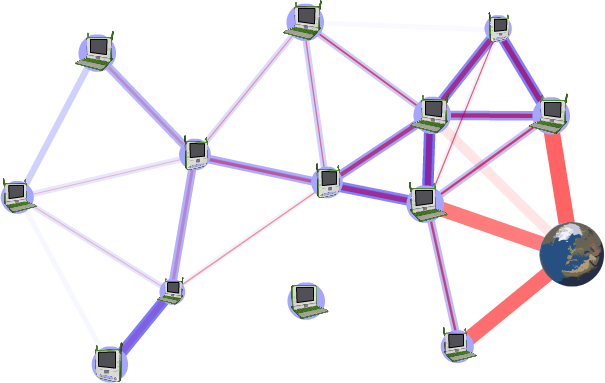
\includegraphics[scale=0.6]{figures/olpc-network}
\par\end{centering}

\caption{\label{fig:OLPC-network-visualization}OLPC network visualization}

\end{figure}


One can drag single laptops on the canvas using the mouse and immediately
observe the effect on the possible connection path changes. The vision
for the current project work was to develop a similar visualization
tool but based on a real network simulation and real packets in order
to be able to observe the choosen routes nearly in realtime.


\subsection{The NS-3 simulator}

The secondary goal was to get accustomed with the NS-3 simulator.
It is supposed to become the successor of the famous NS-2 network
simulator. It is is not backwards compatible and does not rely on
existing NS-2 code. NS-3 is entirely written in C++ and includes state-of-the-art
architectual principles and design patterns. Therefore the current
project work's goal also was to evaluate the usage of the following
technologies supported by NS-3:
\begin{itemize}
\item C++
\item Python
\end{itemize}



\newpage{}


\section{Topology description}


\subsection{Mesh}

The goal of this project was to simulate a simple mesh network. The
assumption for all following simulations is as follows: $n$ Nodes
are directly connected physically together and form a simple network.
The physical connection types being simulated are:
\begin{itemize}
\item \textit{Point-To-Point}: This connection type was chosen because of
its simplicity. It suited well first experiments for setting up the
simulated network. Another consideration was the fact that when more
than two nodes are connected, then the left-most and right-most nodes
are not physically connected (see figure \ref{fig:Point-To-Point-connection-between})
which allowed to experiment with the routing capabilities of NS-3.
\item \textit{Wifi Adhoc}: This connection type was choosen for the final
simulation and for the visioned visualization.
\end{itemize}
%
\begin{figure}
\begin{centering}
% Define two helper counters
\begin{tikzpicture}[auto]

   % % grid
   % \def\supertiny{ \font\supertinyfont = cmr9 at 3pt \relax \supertinyfont}
   % \newcounter{gridrows}
   % \setcounter{gridrows}{12}
   % \newcounter{gridcols}
   % \setcounter{gridcols}{30}
   % \draw [gray, very thin] (0, -\arabic{gridrows}) grid (\arabic{gridcols}, 0);
   % \foreach \x in {0,...,\arabic{gridcols}}
   %     \foreach \y in {0,...,\arabic{gridrows}}
   %     {
   %         \draw (\x+0.15, -\y-0.15) node [gray, very thin] {\supertiny{\x/\y}};
   %     }

    % styles
    \tikzstyle{netnode} = [shape=rectangle, draw, rounded corners=2pt, fill=black!20, minimum height=10mm, minimum width=30mm];
    \tikzstyle{darrow} = [latex-latex];

    \draw 
        node[netnode] (node1) {Node 1}
        node[netnode, right=of node1, xshift=2cm] (node2) {Node 2}
        node[netnode, right=of node2, xshift=2cm] (node3) {Node 3};

    \path
        (node1) edge[darrow] node{Point-To-Point} (node2)
        (node2) edge[darrow] node{Point-To-Point} (node3);
\end{tikzpicture}

\par\end{centering}

\caption{\label{fig:Point-To-Point-connection-between}Point-To-Point connection
between three nodes}

\end{figure}



\subsection{Protocol stack}


\subsubsection{TCP/IP}

The protocol stack being used in all following simulations is standard
TCP/IPv4. Actually it is currently the only protocol stack being supported
by NS-3 at least for the higher OSI levels.


\subsubsection{Routing}

Because the current project emphasizes on the visualization of packets
traveling through a real network, the routing of the packets needs
special attention. In NS-3 currently two rouing models are being supported:
\begin{itemize}
\item \textit{Global Routing}: A static routing table being available at
each node of the network. This table is filled by the NS-3 during
the startup of the target simulation. Obviously this routing method
is only applicable for static, non-moving nodes.
\item \textit{OLSR}\cite{rfc3626}: The Optimized Link State Routing Protocol
is an IP rouing protocol for Adhoc mobile network. This protocol is
being used at the OLPC project and is one of currently available routing
protocols.
\end{itemize}



\newpage{}


\section{The Point-To-Point mesh}


\subsection{\label{sub:Architecture}Architecture}

The NS-3 simulator is heavily based on object-oriented design. Figure
\ref{fig:singlehop} shows a simplified view on a typical NS-3 simulation
architecture, regardless whether programmed in Python or C++.

%
\begin{figure}
\begin{centering}
% Define two helper counters
\begin{tikzpicture}[auto]

   % % grid
   % \def\supertiny{ \font\supertinyfont = cmr9 at 3pt \relax \supertinyfont}
   % \newcounter{gridrows}
   % \setcounter{gridrows}{12}
   % \newcounter{gridcols}
   % \setcounter{gridcols}{30}
   % \draw [gray, very thin] (0, -\arabic{gridrows}) grid (\arabic{gridcols}, 0);
   % \foreach \x in {0,...,\arabic{gridcols}}
   %     \foreach \y in {0,...,\arabic{gridrows}}
   %     {
   %         \draw (\x+0.15, -\y-0.15) node [gray, very thin] {\supertiny{\x/\y}};
   %     }

    % styles
    \tikzstyle{archlayer} = [
        shape=rectangle, 
        draw, 
        rounded corners=2pt, 
        inner sep=0mm, 
        minimum width=30mm, 
        minimum height=10mm,
        fill=blue!20
    ];

    \tikzstyle{darrow} = [latex-latex];

    \node[archlayer] (app) {Application};
    \node[archlayer, fill=yellow!20, below=of app] (stack) {Protocol stack};
    \path (app) edge[darrow] (stack);
    \node[archlayer, fill=green!20, below=of stack] (netdevice) {NetDevice};
    \path (stack) edge[darrow] (netdevice);

    \node[archlayer, fill=red!20, right=of netdevice] (channel) {Channel};
    \path (netdevice) edge[darrow] (channel);

    \node[archlayer, fill=green!20, right=of channel] (netdevice) {NetDevice};
    \path (channel) edge[darrow] (netdevice);
    \node[archlayer, fill=yellow!20, above=of netdevice] (stack) {Protocol stack};
    \path (netdevice) edge[darrow] (stack);
    \node[archlayer, above=of stack] (app) {Application};
    \path (app) edge[darrow] (stack);
\end{tikzpicture}

\par\end{centering}

\caption{Typical NS-3 simulation architecture}



\end{figure}


The following architectual layers can be identified:
\begin{itemize}
\item \textit{Application}: This layer contains the application logic. In
NS-3 one can implement socket-based applications using the internal
NS-3 socket APIs. NS-3 actually also provides operating system dependent
socket implementations (as far as I know the Linux socket API and
the BSD API is supported in NS-3). Finally UDP based applications
are supported and also various helper classes are provided by NS-3
for easy initialization of the application objects. The current project
focuses only on UDP based applications.
\item \textit{Protocol stack}: This architectual layer provides objects
for initializing a concrete protocol stack. Since NS-3 currently only
supports IPv4 only this is the stack the current project relies on.
Furthermore on this layer one specifies the different routing mechanisms
being used by NS-3. The current project uses both supported routing
protocols (static routing and OLSR).
\item \textit{NetDevice}: This layer provides objects for defining the actual
physical layout of the network. In the current project physically
Point-To-Point connections are being examined as well as Wifi connections.
Furthermore this layer provides objects for specifying the actual
positions and movements for the nodes of interest.
\item \textit{Channel}: This layer provides objects the physical communication
channel between nodes. This layer is pretty much hidden from the developer
but hooks and callback methods exists for further analysis and statistics.
\end{itemize}

\subsection{Single Hop simulation}

%
\begin{figure}
\begin{centering}
% Define two helper counters
\begin{tikzpicture}[auto]

   % % grid
   % \def\supertiny{ \font\supertinyfont = cmr9 at 3pt \relax \supertinyfont}
   % \newcounter{gridrows}
   % \setcounter{gridrows}{12}
   % \newcounter{gridcols}
   % \setcounter{gridcols}{30}
   % \draw [gray, very thin] (0, -\arabic{gridrows}) grid (\arabic{gridcols}, 0);
   % \foreach \x in {0,...,\arabic{gridcols}}
   %     \foreach \y in {0,...,\arabic{gridrows}}
   %     {
   %         \draw (\x+0.15, -\y-0.15) node [gray, very thin] {\supertiny{\x/\y}};
   %     }

    % styles
    \tikzstyle{netnode} = [shape=rectangle, draw, rounded corners=2pt, fill=black!20, minimum height=10mm, minimum width=30mm];
    \tikzstyle{darrow} = [latex-latex];

    \draw 
        node[netnode] (node1) {Node 1}
        node[netnode, right=of node1, xshift=3cm] (node2) {Node 2};

    \path
        (node1) edge[darrow] node{Point-To-Point} node[swap]{500kbs, 2ms Delay} (node2);
\end{tikzpicture}

\par\end{centering}

\caption{\label{fig:singlehop}Point-To-Point connection between two nodes}

\end{figure}


The first simulation analyzes two nodes being connected together via
a Point to Point connection. Figure \ref{fig:singlehop} represents
the very simple network being simulated in this case. Listing \ref{lst:singlehop}
shows the relevant Python based program code for this simulation.\texttt{\small \lstinputlisting[breaklines=true,caption={experiment.py (singleHop simulation)},extendedchars=true,firstline=60,label={lst:singlehop},language={Python},lastline=92,numbers=right]{src/sieci/src/experiment.py}}{\small \par}

First a NodeContainer object is being created which instantiates all
simulated nodes of the target network. Afterwards follows a DeviceFactory
which was implemented individually for this project. It initializes
and creates the actual physical devices. Listing \ref{lst:devfactory}
shows the relevant initalization code. One can see that a Point-To-Point
connection between the nodes having a speed of 500kbs and a delay
of 2ms is being initialized.

\texttt{\small \lstinputlisting[breaklines=true,caption={experiment.py (DeviceFactory initialization)},extendedchars=true,firstline=5,label={lst:devfactory},language={Python},lastline=11,numbers=right]{src/sieci/src/experiment.py}}{\small \par}

Afterwards the internet protocol stack is being initialized using
internal NS-3 helper objects. The most important part here is the
assignment of IP addresses to the simulated nodes which is also being
handled by a helper object. Only a base address (here {}``10.0.0.0'')
has to be specified and NS-3 will chronologically assign IP addresses
automatically to all simulated nodes. Here we have two nodes, therefore
the adresses {}``10.0.0.1'' and {}``10.0.0.2'' will be assigned
to the nodes.

At last the actual applications are being initialized using an application
factory developed individually for of this project. The initialization
in Listing \ref{lst:appfactory} install two applications, the sender
application (tx) and the receiver application (rx). Using NS-3 helper
objects an UDP based application is instanciated, which is sending
packets starting at OnTtheime and stopping at OffTime. Here the application
starts sending packets after 1 second of the application start and
never stops sending (OffTime is 0 seconds).

\texttt{\small \lstinputlisting[breaklines=true,caption={experiment.py (ApplicationFactory initialization)},extendedchars=true,firstline=34,label={lst:appfactory},language={Python},lastline=58,numbers=right]{src/sieci/src/experiment.py}}{\small \par}

Since this network consists of only two nodes, it is not necessary
to initialize any routing tables. The two nodes see each other directly.
Python based logging statements were built into the singlehop simulation
and the output can be seen in Listing \ref{lst:singlehoplog}. The
log shows the assigned MAC addresses as well as the dynamically assigned
IP addresses of both nodes.

\texttt{\small \lstinputlisting[breaklines=true,caption={singlehop.log (SingleHop simulation log output)},extendedchars=true,label={lst:singlehoplog}]{src/results/singlehop.log}}{\small \par}

In line 82 and line 84 of lising \ref{lst:singlehop} one can see
that the receiver application starts listening for UDP packets 15
seconds after the beginning of the simulation. The sender application
starts sending UDP packets 5 seconds earlier at the 10th second after
the simulation start. What happens then can be seen best from the
actual packet traces generated by NS-3. It is capable of generating
standard pcap based output files. The pcap trace file can then be
analyzed using existing tools available (i.e. tcpump, wireshark, tcptrace,
etc.). The tcpdump of the generated pcap files can be seen in listing
\ref{lst:singlehoptcpdump}. It can be seen that as long as the receiver
application is not listening for any packets, an ICMP message is being
answered from the receiver node, stating that the application port
is unreachable. Starting from the 15th second the receiver application
then silently accepts the incoming UDP packets.

\texttt{\small \lstinputlisting[breaklines=true,caption={singlehop.tcpdump (SingleHop tcpdump output)},extendedchars=true,label={lst:singlehoptcpdump}]{src/results/singlehop.tcpdump}}{\small \par}


\subsection{Dual Hop simulation using OLSR}

Using the same code basis from the single hop simulation a further
simulation was developed to examine NS-3's routing table capabilities.
Listing \ref{lst:dualhop_} shows the relevant code fragments. The
simulated network consists of three nodes as represented in figure
\ref{fig:Point-To-Point-connection-between}. The nodes are connected
together using a Point-To-Point connection. One can see, that Node1
and Node3 do not see each other physically. Instead Node2 is initialized
to have two net devices, one connecting to Node1 and the other connecting
to Node3. Thus Node1 and Node3 are transiently connected via Node2.
A routing protocol is needed to successfully propagate any packets
from Node1 to Node3. Lines 140-141 of listing \ref{lst:dualhop_}
show the correspondent OLSR initialization code under NS-3.

Because OLSR needs some time to initialize the start of the sender
application and the receiver application were delayed to the 70th
second (sender) and the 80th second (receiver). If the sender starts
too early, the routing tables would not be initialized yet causing
unroutable packets. That is actually one drawback of dynamic routing
protocols. They need time to build and need time to update themself
by a certain delay.

\texttt{\small \lstinputlisting[breaklines=true,caption={experiment.py (dualHop simulation)},extendedchars=true,firstline=94,label={lst:dualhop_},language={Python},lastline=150,numbers=right]{src/sieci/src/experiment.py}}{\small \par}

For the analysis of the dual hop simulation wireshark has been used
because of its very detailed information depth. NS-3 generates a pcap
file for each net device so for the dual hop simulation the following
pcap files exist:

\begin{center}
\begin{tabular}{|c|c|}
\hline 
Node & pcap files\tabularnewline
\hline
\hline 
Node 1 & \multicolumn{1}{c|}{dualHopOlsr-0-0.pcap}\tabularnewline
\hline 
Node 2 & dualHopOlsr-1-0.pcap\tabularnewline
 & dualHopOlsr-1-1.pcap\tabularnewline
\hline 
Node 3 & dualHopOlsr-2-0.pcap\tabularnewline
\hline
\end{tabular}
\par\end{center}

One can see that Node 2 has two pcap files, one for each of the two
assigned net devices forming a Point-To-Point connection with Node
1 on one side and Node 2 an the other. Listing \ref{lst:dualhop_wireshark}
shows the first two packets from the dualHopOlsr-1-0.pcap file, which
represents the channel between Node 1 (10.0.1.1) and Node 2 (10.0.1.2).
The shown two packets are so called HELLO packets. This message type
is defined in the OLSR RFC \cite{rfc3626} as the message type to
propagate the information that a node is actually existent in the
network. All receiving nodes (at least those who are capable of receiving
these HELLO messages) will then know of the existence of the neighbour
nodes and can build a routing table based on this information. Another
interesting fact is the usage of the MID (Multiple Interface Declaration)
message type in the second packet. This message type is used, when
a node has multiple interfaces, which is the case for Node 2. \texttt{\small \lstinputlisting[breaklines=true,caption={dualHopOlsr-1-0.log (dualHop wireshark dump)},extendedchars=true,label={lst:dualhop_wireshark}]{src/results/dualHopOlsr-1-0.log}}{\small \par}

Figure \ref{fig:IO-Graph-statistics} shows the IO graph of the dual
hop simualation, generated using wireshark. Line 132 and line 133
in Listing \ref{lst:dualhop_} specify that the sender application
is supposed to start transmitting UDP packets from the 80th second
up to the 90th second after the simulation start. This peak of packet
activity can be nicely observed in Figure \ref{fig:IO-Graph-statistics}.
A further observation is that when the application is not sending
data, there is still packet traffic existent. It is visible as small
spikes in the IO graph. When observing the wireshark trace then it
can be concluded that this is traffic generated by the OLSR protocol.
So one can say that OLSR is a proactive routing protocol which constantly
updates himself. There is no need for an external {}``trigger''
which initializes the routing update. Therefore this routing protocol
is also suitable for moving nodes, where neighbour nodes change constantly
and thus also the routing information.

%
\begin{figure}
\begin{centering}
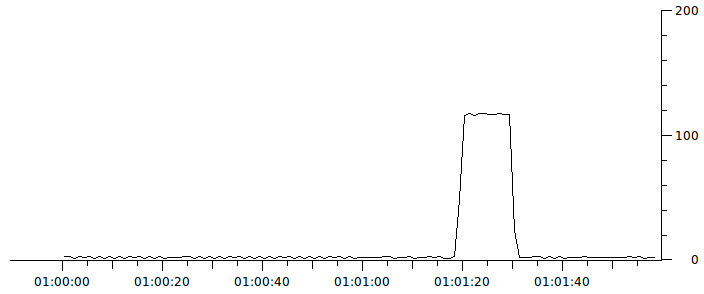
\includegraphics[width=0.7\paperwidth]{src/results/dualHopOlsr}
\par\end{centering}

\caption{\label{fig:IO-Graph-statistics}IO Graph statistics of the dual hop
simulation}

\end{figure}



\newpage{}


\section{The Visualizer}

From the learnings in the first simulations using the Python based
NS-3 API the second part of the project includes the development of
a network visualizer in C++. The architectual principles as described
in chapter \ref{sub:Architecture} also apply to the C++ based API.
Actually the Python based API of NS-3 is a 1:1 mapping of C++ classes
to Python classes using the pybindgen Framework.


\subsection{Dual Hop network visualization}

The main program of the C++ based visualizer is very similar to the
Python based application but ported to C++. Similar to the procedures
in the Python based simulations the first C++ based simulation included
the implementation of a network visualization using only three nodes
as shown in Figure \ref{fig:Point-To-Point-connection-between}. In
addition to the Python based simulations now the simulation includes
real Wifi channels between the nodes instead of simple Point-To-Point
connections. The relevant Wifi initialization is shown in Listing
\ref{lst:wifi_initialization}.

\texttt{\small \lstinputlisting[breaklines=true,caption={wifi-project.cc (wifi initialization)},extendedchars=true,firstline=52,label={lst:wifi_initialization},language={C++},lastline=63,numbers=right]{src/wifi-project/wifi-project.cc}}{\small \par}

Again we generate pcap based trace files (line 61). Furthermore NS-3
helper objects are being used (lines 57-58) to initialize a {}``default''
Wifi model to our simulation. The NS-3 documentation does not clearly
state what the default settings are, so there was some investigation
necessary. Listing \ref{lst:wifilog} shows the log output from the
NS-3 Wifi helper classes. It can be seen that there are pretty lots
of meaningless pointer values in hex format. The only valuable information
is that the Wifi connection has a speed of 6MBit. Clearly this is
a point for enhancement in NS-3 since neither the documentation states
what the default Wifi values are nor the log output (which also has
to be enabled separately). Of course these settings can be programmatically
controlled using the C++ API but the investigation of different Wifi
propagation settings was not part of this project.

\texttt{\small \lstinputlisting[breaklines=true,caption={wifilog.out (log output from NS-3 Wifi helper objects)},extendedchars=true,firstline=1,label={lst:wifilog},lastline=43,numbers=right]{src/results/wifilog.out}}{\small \par}

Since we want to visualize the nodes we have to decide on a positioning
model. NS-3 supports a three-dimensional model using a x-y-z axis
for physically placing nodes. A three-dimensional visualization is
possible using 3D based APIs and there is also a plugin in development
for 3D based NS-3 visualization, but the goal was to implement a similar
visualization to the OLPC flash version as show in Figure \ref{fig:OLPC-network-visualization}
which is clearly based on a simple two-dimensional pane. Therefore
all z-Values were left zero. Listing \ref{lst:dualhop_pos_initialization}
shows the initialization of the physical positions of the three nodes.
The code can be interpreted as follows:
\begin{itemize}
\item line 101: position all nodes on a grid
\item line 102: The minimum x and y location is 10 meters away from the
corner of the simulated pane
\item line 103: The distance between the nodes equals the variable {}``distance'',
which in our case is 100 meters.
\item line 104: The layout type is {}``row first''. That means that the
nodes are being placed automatically in a row first and then, if there
is no place left, one column up.
\end{itemize}
\texttt{\small \lstinputlisting[breaklines=true,caption={wifi-project.cc (position initialization)},extendedchars=true,firstline=99,label={lst:dualhop_pos_initialization},language={C++},lastline=106,numbers=right]{src/wifi-project/wifi-project.cc}}{\small \par}

Similar to the Python based simulations an application logic had to
be implemented. Instead of using built-in NS-3 helper objects an own
application was implemented called wifi-trace which sends UDP packets
every n seconds to the client. The idea was to have bursts of packets
every n seconds which then can be visualized. The relevant sending
logic can be seen in Listing \ref{lst:wifi_trace_sender}.

\texttt{\small \lstinputlisting[breaklines=true,caption={wifi-trace-apps.cc (sender application logic)},extendedchars=true,firstline=115,label={lst:wifi_trace_sender},language={C++},lastline=140,numbers=right]{src/wifi-project/wifi-trace-apps.cc}}{\small \par}

Now in order to visualize a packet route single hops of the packets
traveling through the network have to be catched. NS-3 has a built-in
mechanisms for so called callbacks. Dedicated listener objects can
then be instanciated and can be hooked to listen to callback methods.
Such a listener was implemented in this project and called PacketListener
(defined in packet-listener.cc/packet-listener.h). The callbacks defined
in this project can be seen in Listing \ref{lst:callback_init_}.

\texttt{\small \lstinputlisting[breaklines=true,caption={wifi-project.cc (callback initialization)},extendedchars=true,firstline=133,label={lst:callback_init_},language={C++},lastline=136,numbers=right]{src/wifi-project/wifi-project.cc}}{\small \par}

In Listing \ref{lst:callback_init_} the following two callback methods
are initialized:
\begin{itemize}
\item \textit{Sender}: Whenever a new packet is being transmitted by the
sender application the listener has to be notified about this fact.
The method being triggered is called PacketListener::TxCallback as
shown in Listing \ref{lst:tx_callback}. The listener then stores
the id of the packet in a hashmap (line 66) and knows that a new transmission
is starting.
\item \textit{In-between hop nodes}: Whenever a node is being used as a
router by the OLSR protocol in order to forward a packet to its destination
then the listener has to be notified about this fact. The method being
triggered here is called PacketListener::RxCallback as shown in Listing
\ref{lst:rx_callback_}. The connection of the current node and the
previous node (line 116) can then be drawn as a part of the whole
routing graph in the visualization.
\end{itemize}
\texttt{\small \lstinputlisting[breaklines=true,caption={packet-listener.cc (TxCallback)},extendedchars=true,firstline=64,label={lst:tx_callback},language={C++},lastline=70,numbers=right]{src/wifi-project/packet-listener.cc}}{\small \par}

\texttt{\small \lstinputlisting[breaklines=true,caption={packet-listener.cc (RxCallback)},extendedchars=true,firstline=103,label={lst:rx_callback_},language={C++},lastline=118,numbers=right]{src/wifi-project/packet-listener.cc}}{\small \par}

The visualized packet route is not displayed in realtime during the
simulation but rather logged to a special file. This file is being
interpreted by a newly available NS-3 plugin called {}``Decorator
API'' . The result of the dual-hop visualization can be seen in
Figure \ref{fig:Dual-Hop-visualization}. The pink line represents
an UDP packet travelling via all intermediate nodes forming a route
graph.

%
\begin{figure}
\begin{centering}
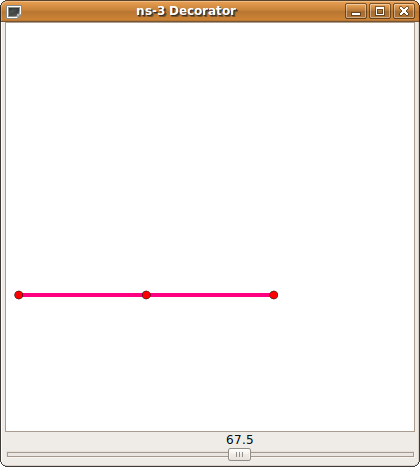
\includegraphics[scale=0.5]{src/results/dualhop_visualization}
\par\end{centering}

\caption{\label{fig:Dual-Hop-visualization}Dual Hop visualization}



\end{figure}



\subsection{Grid network visualization}

Based on the learnings from the Dual Hop visualization and the first
Pyhton based simulations now the final goal was to implement a visualization
of a grid of nodes. It was assumed that the lowest left-most node
is the sender node. Then a receiver node is walking across a grid
of other nodes starting from the middle of the pane. It was assumed
that due to the nature of the OLSR protocol the route graph would
then adapt itself targetting the current position of the walking node.
The distance between all nodes was set up to 100 meters so there was
no danger of a direct connection between the sender and the receiver
node because the distance would be too far.

Listing \ref{lst:grid_network} shows the central simulation code
for the grid simulation. Lines 146-163 initialize the target nodes.
One can see, that a total of 17 nodes is being created. 16 nodes a
are forming a 4x4 grid. The 17th node is the walking node. Lines 169-190
initilialize the mobility model of the 16 grid nodes. The following
properties were programmed for the grid nodes:
\begin{itemize}
\item \textit{Grid positions}: The grid nodes are placed in a grid. A helper
object called ns3::GridPositionAllocator was used to achieve the grid
layout.
\item \textit{Constant positiions}: The grid nodes are node supposed to
move. Therefore a helper object called ns3::ConstantPositionMobilityModel
was used to initalize the grid nodes.
\end{itemize}
Afterwards the moving node is being initialized with the following
properties:
\begin{itemize}
\item Middle start position: The walking node starts from the middle of
the grid pane. Lines 192-195 specify the concrete x-y start position.
\item Random walking: The walking node randomly walks inside the grid. Lines
197-199 specify the random walk model using a helper object called
ns3::RandomWalk2dMobilityModel.
\end{itemize}
Lines 204-208 initialize the Decorator API to be able to visualize
the routing graph. Lines 211-222 initialize the sender and receiver
application. Lines 224-226 initialize the already describe packet
listener. Finally the already discussed callbacks are being initialized
and the simulation starts.

\texttt{\small \lstinputlisting[breaklines=true,caption={wifi-project.cc (grid simulation)},extendedchars=true,firstline=146,label={lst:grid_network},language={C++},lastline=243,numbers=right]{src/wifi-project/wifi-project.cc}}{\small \par}

%
\begin{figure}
\hfill{}\subfloat[53.4th second]{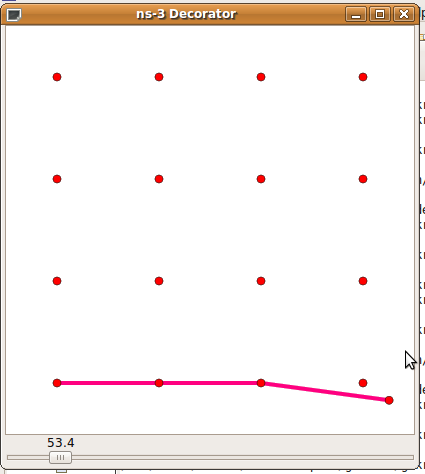
\includegraphics[scale=0.3]{src/results/Screenshot}



}\hfill{}\subfloat[130.4th second]{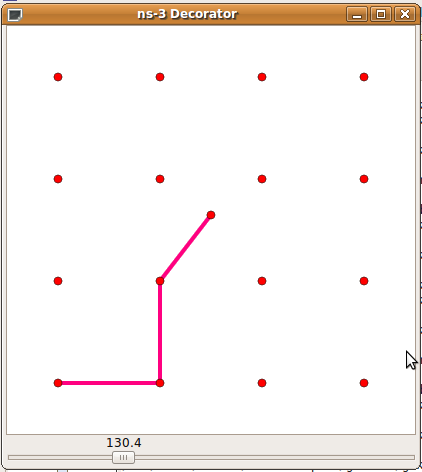
\includegraphics[scale=0.3]{src/results/Screenshot-1}

}\hfill{}

\hfill{}\subfloat[207.4th second]{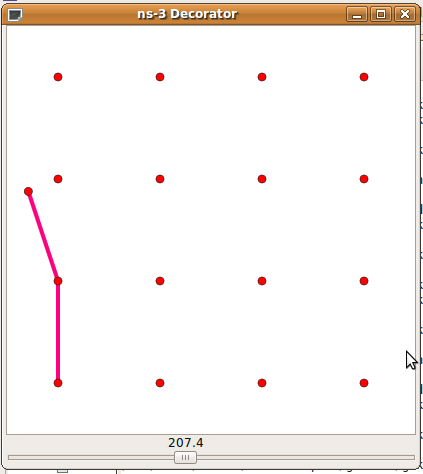
\includegraphics[scale=0.3]{src/results/Screenshot-2}

}\hfill{}\subfloat[263.3th second]{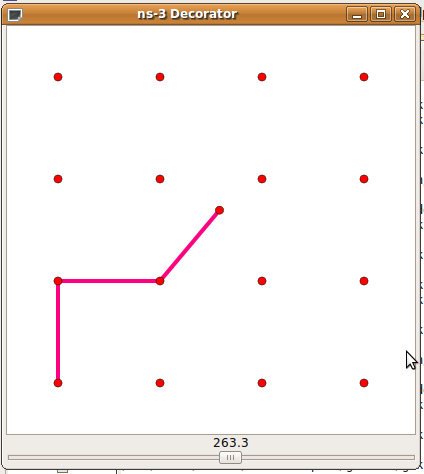
\includegraphics[scale=0.3]{src/results/Screenshot-3}

}\hfill{}

\hfill{}\subfloat[319.1th second]{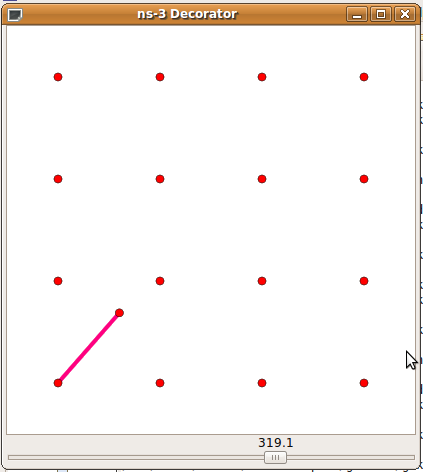
\includegraphics[scale=0.3]{src/results/Screenshot-4}

}\hfill{}\subfloat[408.5th second]{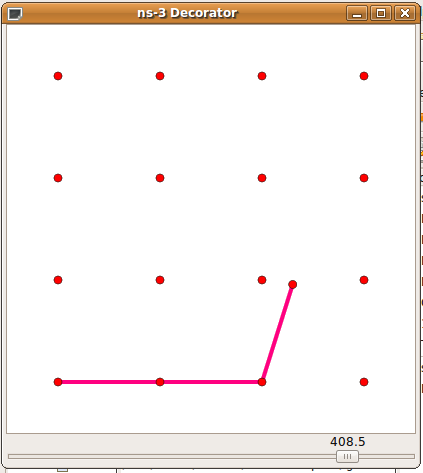
\includegraphics[scale=0.3]{src/results/Screenshot-5}

}\hfill{}

\hfill{}\subfloat[445.8th second]{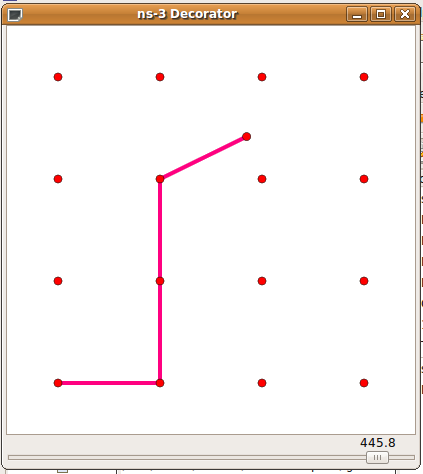
\includegraphics[scale=0.3]{src/results/Screenshot-6}

}\hfill{}\subfloat[466.9th second]{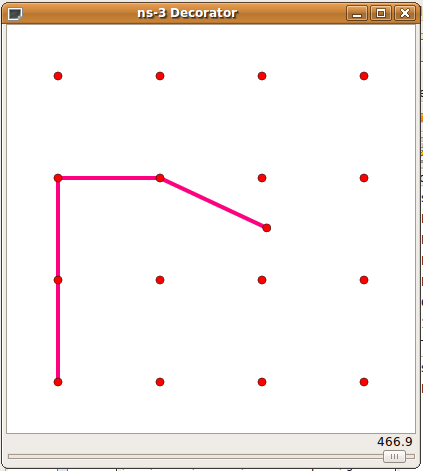
\includegraphics[scale=0.3]{src/results/Screenshot-7}

}\hfill{}

\caption{\label{fig:The-grid-network}The grid network visualization}



\end{figure}


Figure \ref{fig:The-grid-network} shows single snapshops of the overall
visualized simulation at different time points. One can see how the
receiver node walks randomly amongst the grid of router node.


\newpage{}


\section{Conclusions}

All envisioned goals were successfully realized in this project. Nevertheless
NS-3 is still in development and implies a steep learning curve. The
Decorator API used for this project is not in the main tree of the
NS-3 project yet. Furthermore the Python bindings were not available
for the Decorator API and the biggest drawback is that the current
Python binding does not support callbacks yet. Therefore a switch
from Python to C++ actually was necessary to successfully complete
the project.


\newpage{}

\listoffigures


\newpage{}
\begin{thebibliography}{2}
\bibitem{olpc-website}The OLPC website:\\
\url{http://www.olpc.org}

\bibitem{rfc3626}RFC 3626\\
\url{http://www.ietf.org/rfc/rfc3626.txt}
\end{thebibliography}

\end{document}
